% Uncomment this to make slides with overlays:
\documentclass[slides]{beamer}

% Uncomment these (but comment the above \documentclass line) to make handouts:
%\documentclass[handout]{beamer}

% Uncomment these to have more than one slide per page
%\usepackage{pgfpages}
%\pgfpagesuselayout{2 on 1}[border shrink=5mm]
%\pgfpageslogicalpageoptions{1}{border code=\pgfusepath{stroke}}
%\pgfpageslogicalpageoptions{2}{border code=\pgfusepath{stroke}}

\usepackage[]{graphicx, color, hyperref}

\mode<presentation>
{
	%\usetheme[secheader]{Boadilla}
	%\usecolortheme[rgb={.835, .102,.169}]{structure}  
	\usetheme[width= 0cm]{Goettingen}
	%\setbeamercovered{transparent}
}
\setbeamertemplate{navigation symbols}{}
\setbeamertemplate{footline}[frame number]

\definecolor{blue2}{rgb}{0.278,0.278,0.729} 
\newcommand{\blue}[1]{\textcolor{blue2}{#1}}
\newcommand{\white}[1]{\textcolor{white}{#1}}
\newcommand{\grey}[1]{\textcolor{grey}{#1}}
\newcommand{\red}[1]{\textcolor{red}{#1}}
\newcommand{\xbar}{\overline{x}}
\newcommand{\ybar}{\overline{y}}
\newcommand{\phat}{\widehat{p}}
\newcommand{\prob}{\mbox{Pr}}
\newcommand{\E}{\mathbb{E}}
\newcommand{\Var}{\mbox{Var}}
\newcommand{\cp}{\oplus}
\newcommand{\cm}{\circleddash}


\title{Lecture 28: Logistic Regression}
\author{Chapter 8.4}
\date{}


\begin{document}
%------------------------------------------------------------------------------
\begin{frame}
\titlepage
\end{frame}
%------------------------------------------------------------------------------


%library(openintro)
%data(email)
%model <- glm(spam~to_multiple+winner+format+re_subj+attach+password, family=binomial, data=email)
%
%pdf("./13.1 Logistic Regression/fitted.pdf", width=5, height=5)
%hist(fitted(model), xlab="fitted probabilities", main="")
%dev.off()
%
%
%pdf("./13.1 Logistic Regression/fitted2.pdf", width=5, height=5)
%hist(fitted(model), xlab="fitted probabilities", main="")
%abline(v=0.65, col="red", lwd=2)
%dev.off()
%
%ftable(spam=email$spam, class=fitted(model)>0.65)
%
%
%pdf("./13.1 Logistic Regression/fitted3.pdf", width=5, height=5)
%hist(fitted(model), xlab="fitted probabilities", main="")
%abline(v=0.3, col="red", lwd=2)
%dev.off()
%
%ftable(spam=email$spam, class=fitted(model)>0.3)


%------------------------------------------------------------------------------
\begin{frame}[fragile]
\frametitle{Binary Outcome Variables}

%
% Comment this
%
%Instead of numerical outcomes, we have observations $Y_i$ for $i=1,\ldots,n$ where
%\begin{itemize}
%\item $Y_i=1$ with probability $p_i$
%\item $Y_i=0$ with probability $1-p_i$
%\end{itemize}
%
%\vspace{0.5cm}
%\pause
%\blue{Logistic regression}: we are modeling $p_i$'s with a linear model.

\end{frame}
%------------------------------------------------------------------------------


%------------------------------------------------------------------------------
\begin{frame}[fragile]
\frametitle{Outcome Variable}

%
% Comment this
%
%Let
%\[
%x_{1,i}, \ldots x_{k,i}
%\]
%be the $k$ predictor variables associated with the $i^{th}$ observation
%
%\vspace{0.5cm}
%\pause
%One's first thought might be to model the $p_i$'s using linear regression:
%
%\[
%p_i = \beta_0 + \beta_1 x_{1,i} + \ldots + \beta_k x_{k,i}
%\]
%
%\vspace{0.5cm}
%\pause
%However, you may end up fitting $p_i$'s that are either
%\begin{itemize}
%\item less than 0
%\item greater than 1
%\end{itemize}

\end{frame}
%------------------------------------------------------------------------------


%------------------------------------------------------------------------------
\begin{frame}[fragile]
\frametitle{Logit Transformation}

%
% Comment this
%
%Rather, what is modeled is the \blue{logit transformation} or \blue{log-odds} of $p_i$
%\[
%\mbox{logit}(p_i) = \log\left(
%\frac{p_i}{1-p_i}
%\right) = \beta_0 + \beta_1 x_{1,i} + \ldots + \beta_k x_{k,i}
%\]
%\pause
%Why this transformation?  It maps the $[0,1]$ interval to a $(-\infty, \infty)$ interval.  

\end{frame}
%------------------------------------------------------------------------------


%------------------------------------------------------------------------------
\begin{frame}[fragile]
\frametitle{Odds}

%
% Comment this
%
%First, convert $p_i$ into odds:
%
%\vspace{0.25cm}
%
%``Two to one odds for event X'' $\equiv$ ``There is a 66\% chance of event X occurring.''
%
%\pause \vspace{0.25cm}
%
%
%Then we take the natural log of it.  So
%\begin{itemize}
%\pause\item for $p_i=0 \Rightarrow \log\left(\frac{p_i}{1-p_i}\right) = \log\left(\frac{0}{1}\right) = -\infty$
%%------------
%\pause\item for $p_i=0.5 \Rightarrow \log\left(\frac{p_i}{1-p_i}\right) = \log\left(\frac{0.5}{0.5}\right) = 0$
%%------------
%\pause\item for $p_1=1  \Rightarrow \log\left(\frac{p_i}{1-p_i}\right) = \log\left(\frac{1}{0}\right) = \log(\infty) = \infty$
%%\footnote{Not defined actually, we need to state $\lim_{p_i \rightarrow 1}\frac{p_i}{1-p_i}=\infty$} 
%\end{itemize}

\end{frame}
%------------------------------------------------------------------------------


%------------------------------------------------------------------------------
\begin{frame}[fragile]
\frametitle{Outcome Variable}
Figure 8.13 from page 388

\vspace{6cm}

\end{frame}
%------------------------------------------------------------------------------


%------------------------------------------------------------------------------
\begin{frame}[fragile]
\frametitle{Simple Logistic Regression Example p.388}

So say we fit a logistic regression with:
\begin{itemize}
\item $Y_i$ is {\tt spam}:  binary variable of whether message was classified as spam (1 if spam)
\pause\item $x_i$ is {\tt to\_multiple}:  binary variable indicating if more than one recipient listed
\end{itemize}
\pause
\begin{table}[ht]
\centering
\begin{tabular}{r|rrrr}
  \hline
 & Estimate & Std. Error & z value & Pr($>$$|$z$|$) \\ 
  \hline
(Intercept) & -2.1161 & 0.0562 & -37.67 & 0.0000 \\ 
  {\tt to\_multiple} & -1.8092 & 0.2969 & -6.09 & 0.0000 \\ 
   \hline
\end{tabular}
\end{table}

%
% Comment this
%
%The regression equation is
%\[
%\log\left(\frac{p_i}{1-p_i}\right) = -2.12 - 1.81 \times {\tt to\_multiple} 
%\]

\end{frame}
%------------------------------------------------------------------------------


%------------------------------------------------------------------------------
\begin{frame}[fragile]
\frametitle{Inverse Logit Transformation}
%
% Comment this
%
%How do we convert back into $p_i$'s?
%\pause
%\begin{eqnarray*}
%\mbox{Say } x = \log\left(\frac{p_i}{1-p_i}\right) \mbox{ then } p_i = \frac{\exp(x)}{1 + \exp(x)}
%\end{eqnarray*}
%is the \blue{inverse logit transformation}.
%
%\vspace{0.5cm}
%\pause
%So to convert the regression equation to probabilities, we compute
%
%\begin{eqnarray*}
%%p_i &=& \frac{\exp(\beta_0 + \beta_1 x_{1,i} + \ldots + \beta_k x_{k,i})}{1 + \exp(\beta_0 + \beta_1 x_{1,i} + \ldots + \beta_k x_{k,i})}
%p_i &=& \frac{1}{1 + \exp(-(\beta_0 + \beta_1 x_{1,i} + \ldots + \beta_k x_{k,i}))}
%\end{eqnarray*}


\end{frame}
%------------------------------------------------------------------------------


%------------------------------------------------------------------------------
\begin{frame}[fragile]
\frametitle{Fitted Probabilities}
%
% Comment this
%
%To compute the fitted probabilities $\widehat{p}_i$:
%\begin{itemize}
%\item {\tt to\_multiple}$ = 0$ (only one recipient):
%\[
%%\widehat{p}_i = \frac{\exp(-2.12 - 1.81 \times 0)}{1 + \exp(-2.12 - 1.81 \times 0)} = 0.11
%\widehat{p}_i = \frac{1}{1 + \exp(-(-2.12 - 1.81 \times 0))} = 0.11
%\]
%\item {\tt to\_multiple}$ = 1$ (many recipients):
%\[
%%\widehat{p}_i = \frac{\exp(-2.12 - 1.81 \times 1)}{1 + \exp(-2.12 - 1.81 \times 1)} = 0.02
%\widehat{p}_i = \frac{1}{1 + \exp(-(-2.12 - 1.81 \times 1))} = 0.02
%\]
%\end{itemize}
%\pause
%Note:  11\% and 2\% are not dramatically different.  In an ideal world of binary predictors, we'd have fitted probabilities of 100\% and 0\%.
\end{frame}
%------------------------------------------------------------------------------


%------------------------------------------------------------------------------
\begin{frame}[fragile]
\frametitle{Fitted Model Using Backwards Regression}
The following model was selected in the text using backwards selection using $\alpha=0.05$.

\begin{table}[ht]
\centering
\begin{tabular}{r|rrrr}
  \hline
 & Estimate & Std. Error & z value & Pr($>$$|$z$|$) \\ 
  \hline
(Intercept) & -0.8057 & 0.0880 & -9.15 & 0.0000 \\ 
  to\_multiple? & -2.7514 & 0.3074 & -8.95 & 0.0000 \\ 
  word winner used? & 1.7251 & 0.3245 & 5.32 & 0.0000 \\ 
  special formatting? & -1.5857 & 0.1201 & -13.20 & 0.0000 \\ 
  `RE:' in subject? & -3.0977 & 0.3651 & -8.48 & 0.0000 \\ 
  attachment? & 0.2127 & 0.0572 & 3.72 & 0.0002 \\ 
  word password used? & -0.7478 & 0.2956 & -2.53 & 0.0114 \\ 
   \hline
\end{tabular}
\end{table} 

\end{frame}
%------------------------------------------------------------------------------


%------------------------------------------------------------------------------
\begin{frame}[fragile]
\frametitle{Fitted Model Using Backwards Regression}
The following variables increase the probability that the email is spam, since $b>0$

\begin{table}[ht]
\centering
\begin{tabular}{r|rrrr}
  \hline
 & Estimate & Std. Error & z value & Pr($>$$|$z$|$) \\ 
  \hline
(Intercept) & -0.8057 & 0.0880 & -9.15 & 0.0000 \\ 
  \white{to\_multiple?} & \white{-2.7514} & \white{0.3074} & \white{-8.95} & \white{0.0000} \\ 
  \blue{word winner used?} & \blue{1.7251} & \blue{0.3245} & \blue{5.32} & \blue{0.0000} \\ 
  \white{special formatting?} & \white{-1.5857} & \white{0.1201} & \white{-13.20} & \white{0.0000} \\ 
  \white{`RE:' in subject?} & \white{-3.0977} & \white{0.3651} & \white{-8.48} & \white{0.0000} \\ 
  \blue{attachment?} & \blue{0.2127} & \blue{0.0572} & \blue{3.72} & \blue{0.0002} \\ 
  \white{word password used?} & \white{-0.7478} & \white{0.2956} & \white{-2.53} & \white{0.0114} \\ 
   \hline
\end{tabular}
\end{table} 

\end{frame}
%------------------------------------------------------------------------------


%------------------------------------------------------------------------------
\begin{frame}[fragile]
\frametitle{Fitted Model Using Backwards Regression}
The following variables decrease the probability that the email is spam, since $b<0$

\begin{table}[ht]
\centering
\begin{tabular}{r|rrrr}
  \hline
 & Estimate & Std. Error & z value & Pr($>$$|$z$|$) \\ 
  \hline
(Intercept) & -0.8057 & 0.0880 & -9.15 & 0.0000 \\ 
  \blue{to\_multiple?} & \blue{-2.7514} & \blue{0.3074} & \blue{-8.95} & \blue{0.0000} \\ 
  \white{word winner used?} & \white{1.7251} & \white{0.3245} & \white{5.32} & \white{0.0000} \\ 
  \blue{special formatting?} & \blue{-1.5857} & \blue{0.1201} & \blue{-13.20} & \blue{0.0000} \\ 
  \blue{`RE:' in subject?} & \blue{-3.0977} & \blue{0.3651} & \blue{-8.48} & \blue{0.0000} \\ 
  \white{attachment?} & \white{0.2127} & \white{0.0572} & \white{3.72} & \white{0.0002} \\ 
  \blue{word password used?} & \blue{-0.7478} & \blue{0.2956} & \blue{-2.53} & \blue{0.0114} \\ 
   \hline
\end{tabular}
\end{table} 

\end{frame}
%------------------------------------------------------------------------------


%------------------------------------------------------------------------------
\begin{frame}[fragile]
\frametitle{Fitted Probabilities}
These are all 3921 fitted probabilities $\widehat{p}$:
\begin{center}
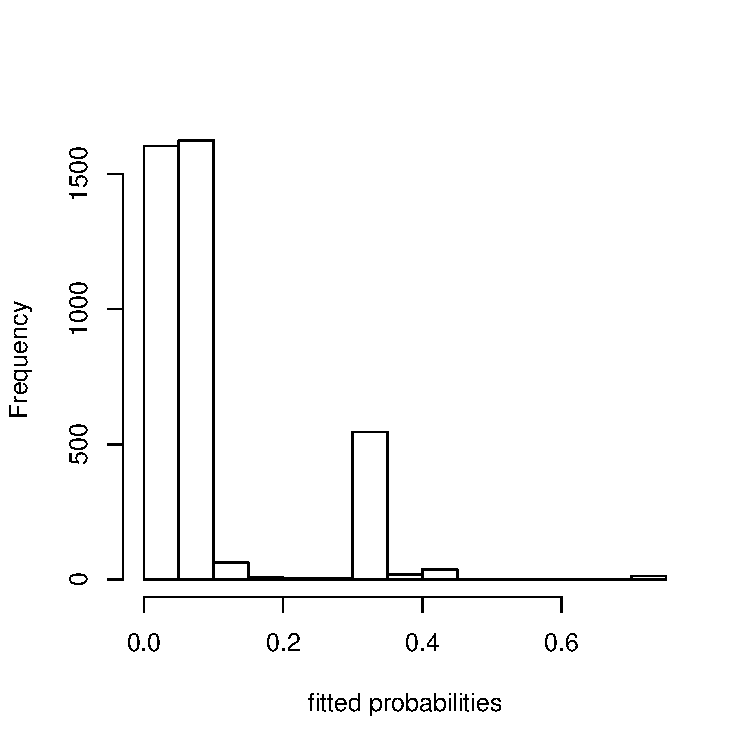
\includegraphics[width=3in]{figure/fitted.pdf}
\end{center}

\end{frame}
%------------------------------------------------------------------------------


%------------------------------------------------------------------------------
\begin{frame}[fragile]
\frametitle{Using Cutoffs to Classify Emails as Spam}

Say we use a cutoff of 65\% to \blue{classify} an email spam or not:
\begin{center}
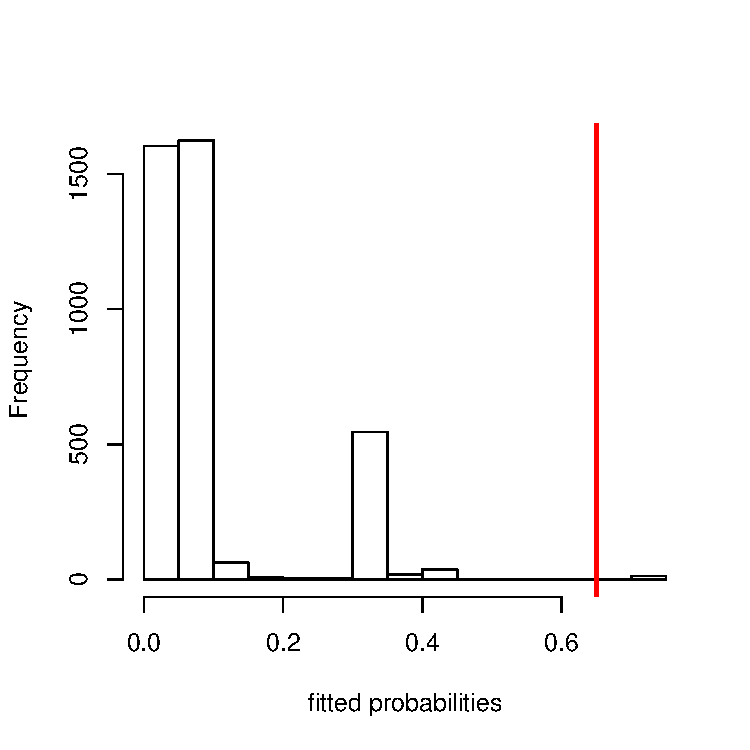
\includegraphics[width=3in]{figure/fitted2.pdf}
\end{center}

\end{frame}
%------------------------------------------------------------------------------


%------------------------------------------------------------------------------
\begin{frame}[fragile]
\frametitle{Using Cutoffs to Classify Emails as Spam}

Using a cutoff of 65\%:
\begin{center}
  \begin{tabular}{cr|cc}
     \multicolumn{2}{c}{}  & \multicolumn{2}{c}{\textbf{Classification}} \\ 
     &  & Not Spam & Spam \\ 
     &  & $\widehat{p}_i < .65$ & $\widehat{p}_i \geq .65$ \\ 
\hline
    \textbf{Truth} & Not Spam: $Y_i=0$ & 3351 & 3\\
     & Spam: $Y_i=1$ & 357 & 10\\ 
    \hline
  \end{tabular}
\end{center}
%
% Comment this
%
%\pause
%\begin{itemize}
%\item Of the emails classified as spam:  $\frac{10}{10+3} = 76\%$ correct
%\item Of the emails classified not as spam:  $\frac{3351}{3351+357} = 90.3\%$ correct
%\end{itemize}


\end{frame}
%------------------------------------------------------------------------------


%------------------------------------------------------------------------------
\begin{frame}[fragile]
\frametitle{Using Cutoffs to Classify Emails as Spam}

Now say we use a cutoff of 30\% to \blue{classify} an email spam or not:
\begin{center}
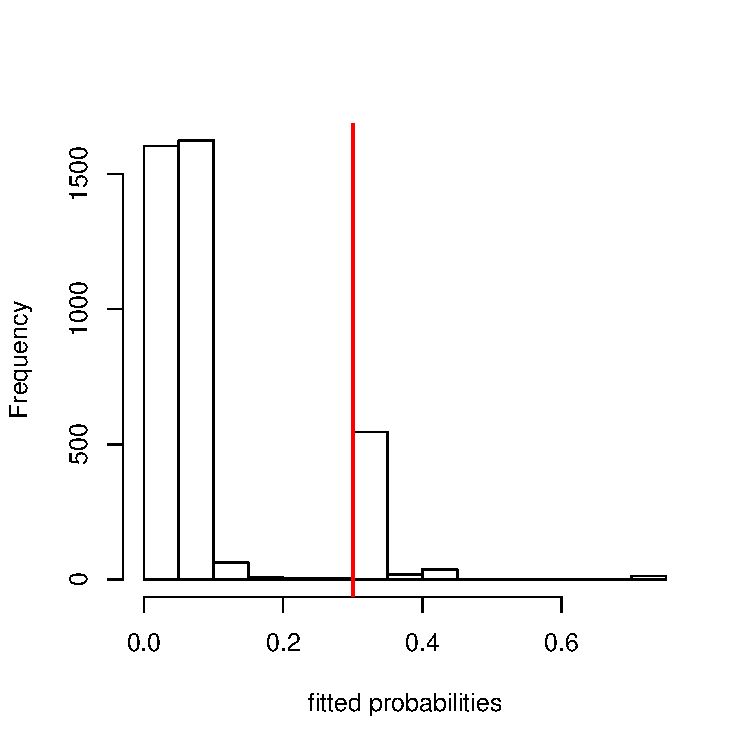
\includegraphics[width=3in]{figure/fitted3.pdf}
\end{center}

\end{frame}
%------------------------------------------------------------------------------


%------------------------------------------------------------------------------
\begin{frame}[fragile]
\frametitle{Using Cutoffs to Classify Emails as Spam}

Using a cutoff of 30\%:
\begin{center}
  \begin{tabular}{cr|cc}
     \multicolumn{2}{c}{}  & \multicolumn{2}{c}{\textbf{Classification}} \\ 
     &  & Not Spam & Spam \\ 
     &  & $\widehat{p}_i < .30$ & $\widehat{p}_i \geq .30$ \\      
\hline
    \textbf{Truth} & Not Spam: $Y_i=0$ & 3138 & 416\\
     & Spam: $Y_i=1$ & 166 & 201\\ 
    \hline
  \end{tabular}
\end{center}
%
% Comment this
%
%\pause
%\begin{itemize}
%\item Of the emails classified as spam:  $\frac{201}{201+416} = 32.6\%$ correct
%\item Of the emails classified not as spam:  $\frac{3138}{3138+166} = 95.0\%$ correct
%\end{itemize}

\end{frame}
%------------------------------------------------------------------------------


%------------------------------------------------------------------------------
\begin{frame}[fragile]
\frametitle{Using Cutoffs to Classify Emails as Spam}

%
% Comment this
%
%\blue{Moral of the Story}:  most classifiers are never perfect (like hypothesis tests).  There will almost always be a trade-off between:  
%\begin{itemize}
%\item Type I errors:  labeling an email spam when it is not
%\item Type II errors:  failing to label an email as spam when it is 
%\end{itemize}

\end{frame}
%------------------------------------------------------------------------------


%------------------------------------------------------------------------------
\begin{frame}[fragile]
\frametitle{Conditions for Logistic Regression}

%
% Comment this
%
%\begin{itemize}
%\item There is a roughly linear relationship between each of the predictors and $\log\left(\frac{p}{1-p}\right)$.
%\pause\item Each outcome $Y_i$ is independent of the other outcomes.
%\end{itemize}
%
%\pause Please read pages 375 and 376 from the text.  

\end{frame}
%------------------------------------------------------------------------------



\end{document}










